\documentclass{article}

\PassOptionsToPackage{numbers,sort&compress}{natbib}
\usepackage[preprint]{neurips_2026}

\usepackage[utf8]{inputenc} % allow utf-8 input
\usepackage[T1]{fontenc}    % use 8-bit T1 fonts
\usepackage{hyperref}       % hyperlinks
\usepackage{url}            % simple URL typesetting
\usepackage{booktabs}       % professional-quality tables
\usepackage{amsfonts}       % blackboard math symbols
\usepackage{nicefrac}       % compact symbols for 1/2, etc.
\usepackage{microtype}      % microtypography
\usepackage{xcolor}         % colors
\usepackage{graphicx}
\usepackage{array}

% XeTeX (tectonic): Times-style Unicode font, plus CJK glyphs for the author line and reference entries
\usepackage{fontspec}
\setmainfont{texgyretermes}[Extension=.otf,UprightFont=*-regular,BoldFont=*-bold,ItalicFont=*-italic,BoldItalicFont=*-bolditalic]
\usepackage{xeCJK}
\setCJKmainfont{Songti SC}
\setCJKmonofont{Songti SC}
\xeCJKsetup{CJKmath=true}

\hypersetup{colorlinks=true,linkcolor=black,citecolor=blue!60!black,urlcolor=blue!60!black}

\title{Recursive Self-Improvement in AI: A Survey of Claims, Evidence, and Empirical Tests}

\author{%
  Qi Sun (孙祺)
}

\begin{document}

\maketitle

\begin{abstract}
AI systems can improve models, code, and training pipelines. Evidence for recursive self-improvement (RSI) requires a further result: successors must become faster at improving under comparable conditions. A review of four public reports and the related literature found no controlled weight-level comparison of this kind. In a three-hour NanoChat run, Qwen3.5-9B lowered validation loss from 1.4152 to 1.2308 across 72 attempts. Yet fine-tuning on its research records and letting it design update recipes did not produce a faster successor across three generations. This report defines the measurement gap, tests it on eight unseen tasks, and outlines how Ling could train against successor improvement speed~\cite{E-28,lit-rsi-academic-md,LOG-E,decisions-decisions-1420-json}.
\end{abstract}

%=====================================================================
\section{Introduction}

AI systems now help develop models, code, and training pipelines. Recursive self-improvement (RSI) makes a stronger claim: the system changes its own improvement mechanism, and successive generations improve faster~\cite{T-05,T-12,T-24}.

This report reviews theoretical definitions, related academic work, and four public reports from Recursive, Naive, and Apex. These reports describe AI improving training code, inference systems, model architectures, or training data. They do not show whether a successor becomes a faster improver. This review found no controlled measurement of this kind at the level of model weights~\cite{E-28}\cite[\S1, \S6]{lit-rsi-academic-md}.

To examine that gap, Qwen3.5-9B first conducted research on NanoChat; successors were then trained on its research records, and their improvement speed was compared across eight unseen micro-research tasks. The fixed original model achieved a clear first-order improvement, lowering NanoChat validation loss from 1.4152 to 1.2308. Across generations, none of the three successors improved faster than the original, and fine-tuning on accepted records did not outperform a placebo trained on rejected records~\cite{LOG-E,decisions-decisions-1420-json}. A lessons note written from the model's own experience reduced improvement speed by about a third and underperformed generic advice on all eight tasks. Letting the model design its training recipe also produced no reliable acceleration (Figure~\ref{fig:forest})~\cite{LOG-E,decisions-decisions-1420-json}. 



\begin{figure}[t]
  \centering
  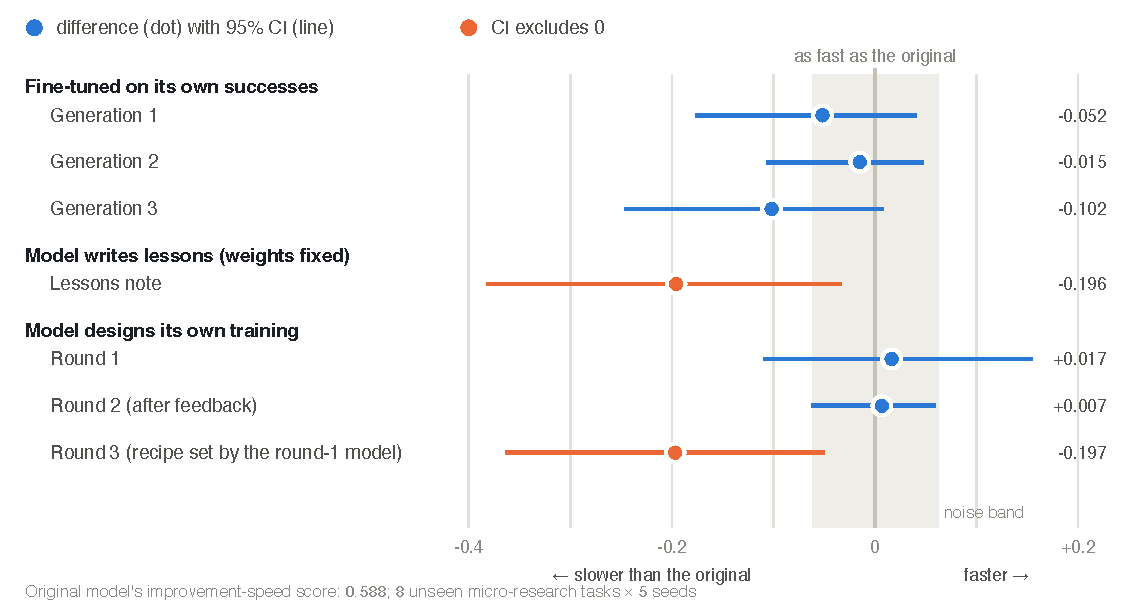
\includegraphics[width=0.72\linewidth]{figs/fig0-forest.pdf}
  \caption{Does a successor improve faster? Each row shows one update method. The dot is its difference in improvement-speed score from the original Qwen3.5-9B, with a 95\% confidence interval. The shaded band shows baseline variation when the original model runs twice ($\pm$2 SD). A value left of zero means slower improvement. Scores come from eight unseen micro-research tasks~\cite{LOG-E,decisions-decisions-1420-json}.}
  \label{fig:forest}
\end{figure}
%=====================================================================
\section{What RSI requires}
\label{sec:rsi}

In 1965, I.\,J.~Good argued that a machine capable of surpassing humans across intellectual tasks should also be able to design better machines; successors repeating this process could trigger an ``intelligence explosion''~\cite{T-01}. The idea became known as recursive self-improvement, but researchers still disagree on its boundaries. An ICLR workshop devoted to RSI in 2026 likewise stopped short of a general formal definition~\cite{T-23}.

The central question is whether the improvement loop returns to the improver. Yudkowsky distinguishes a system optimizing itself from one system optimizing a separate object~\cite{T-03,T-12}. A fixed model that repeatedly improves training code or a target model makes first-order research progress. The loop becomes recursive when an updated system takes over as the researcher and changes its own capacity to make further improvements.

Two questions are often bundled together: who controls the improvement mechanism, and whether improvement accelerates across generations. Tang et al.\ use the first as a formal boundary. When data selection, training recipes, or other mechanisms remain outside the agent, the process is general iterative policy improvement (GPI); it qualifies as RSI under their definition only when the system can internalize and rewrite those mechanisms~\cite{T-24}. This definition classifies the mechanism; evidence of effectiveness requires a separate measurement. Yampolskiy distinguishes self-modification, weak self-improvement, and recursive self-improvement; the highest level requires the system to get better at getting better by improving how it produces successors~\cite{T-12}. Chalmers calls the relevant capacity self-amplifying capacity, the capacity to produce the next generation~\cite{T-09}. Thus, self-distillation or self-play may improve a target task, but if people fix the training process in advance, task scores alone do not establish stronger recursive improvement (an inference)~\cite{T-08,T-12,T-24}.

This report separates the evidence into two levels. \textbf{First-order improvement} occurs when a fixed researcher improves a target under a given budget; Qwen3.5-9B lowering NanoChat validation loss from 1.4152 to 1.2308 is a first-order result~\cite{LOG-E}. \textbf{Second-order improvement} is cross-generation improvement: it compares the speed of successor researchers under the same tasks and budget. A successor that improves faster than its predecessor provides direct evidence that the capacity to improve is growing. Weco calls this threshold ignition, and AIDE$^2$ operationalizes it with an ignition test~\cite{X-24,E-28}; HGM measures an agent's capacity to produce stronger descendants as metaproductivity~\cite{E-27}.

Macro-level work uses the R\&D return parameter $r$ to describe the relation between research input and efficiency. Epoch and Forethought define $r$ in terms of the efficiency gain associated with a doubling of R\&D input; values above 1 correspond to increasingly large efficiency gains per doubling~\cite{T-16,T-17}. Historical estimates vary widely, and no direct estimate is available for LLM research~\cite{T-17}. This report measures generational improvement speed under a fixed budget. It is distinct from $r$, which relates cumulative research input to software efficiency.

%=====================================================================
\section{What the industry reports and the literature show}
\label{sec:evidence}

\subsection{Four industry reports: first-order improvement}

In 2026, Recursive, Naive, and Apex published four reports on AI-assisted R\&D. The reports document what each system improved and how much of the research process it automated (Figure~\ref{fig:disclosure}). Figures below are self-reported by each team.

\begin{figure}[t]
  \centering
  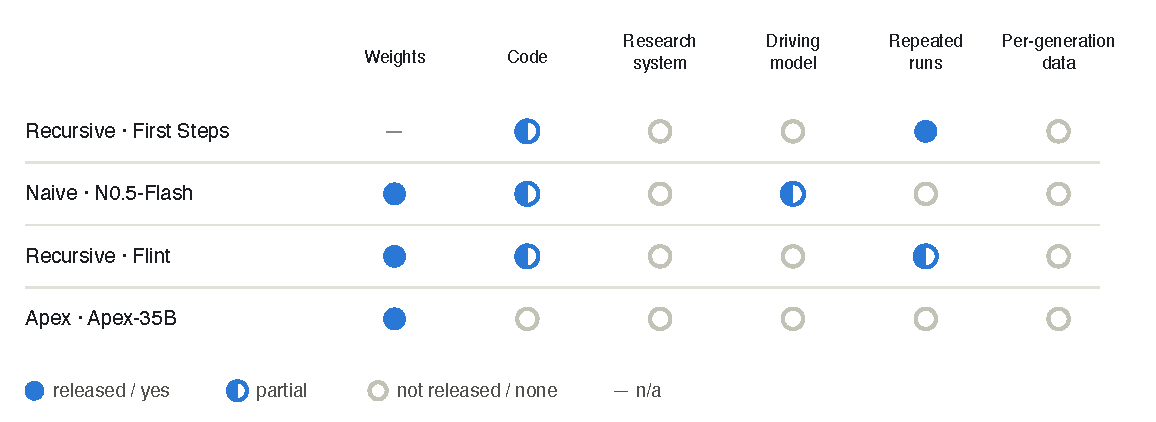
\includegraphics[width=0.70\linewidth]{figs/fig2-disclosure-print.pdf}
  \caption{What the four reports disclose. Filled circles indicate disclosed or available information, half-filled circles partial disclosure, and open circles information that is absent. Based on the reports~\cite{REL-RF,REL-NV,REL-FL,REL-AX}.}
  \label{fig:disclosure}
\end{figure}

\textbf{Recursive, \emph{First Steps Toward Automated AI Research}.} Recursive reports automated improvements to NanoChat training code, NanoGPT Speedrun, and GPU kernels. The system lowered NanoChat validation loss from 0.9372 to 0.9109, reduced Speedrun time from 79.7 to 77.5 seconds, and raised the mean SOL-ExecBench score from 0.699 to 0.754 (self-reported)~\cite{REL-RF}. The results document gains in training code, runtime, and kernel performance. They do not measure whether later researchers improved faster.

\textbf{Naive, \emph{N0.5-Flash}, NaiveRT, and AutoWM.} Naive's report covers model architecture, inference systems, and world-model research. NaiveRT logs 151 optimization attempts and reports reducing speculative decoding time from 12.3 to 3.4 milliseconds; AutoWM, developed with N0.5-Flash, reports a score of 77.43 on WorldArena (self-reported)~\cite{REL-NV}. The report records model contributions to architecture and system optimization, alongside human work. It does not compare the research speed of successive improvers.

\textbf{Recursive, \emph{Flint}.} Flint is a model trained from scratch with help from Recursive's Eureka Machine. Recursive reports its scale, training timeline, and inference efficiency as outcomes of automated R\&D~\cite{REL-FL}. Flint extends automated R\&D to model construction. Recursive presents Flint taking over development of the Eureka Machine as future work~\cite{REL-FL}.

\textbf{Apex, \emph{Apex-35B-V1.0}.} Apex continues training from Qwen3.6-35B-A3B and describes its AI4AI work as recursive self-improvement~\cite{REL-AX}. One example reports that a training procedure designed by Apex raised Qwen2.5-3B-Instruct's success rate on 512 Sokoban levels from 11.7\% to 24.4\% (self-reported)~\cite{REL-AX}. The result shows Apex designing and running an RL experiment. The report does not compare Apex generations on research speed.

The four reports present meaningful first-order results: AI helps improve code, architectures, inference systems, or training procedures, and the target's measured performance improves. They do not provide second-order evidence: placing the updated model in the researcher role and testing whether it improves faster than its predecessor under the same tasks and budget. These are meaningful engineering results. Evidence of recursive improvement requires testing whether the resulting system becomes a faster researcher.

\subsection{The literature: the missing measurement}

Current benchmarks mostly measure whether a model can perform research tasks. RE-Bench evaluates machine-learning engineering, MLE-bench tracks medals in Kaggle competitions, and PaperBench tests paper reproduction~\cite{E-01,E-03,E-04}. They answer what a model can do now. They do not answer whether a successor produced through research can do the same work faster. METR estimates that Anthropic's overall R\&D pace has increased by about 1.9 times, but that figure includes human researchers and cannot isolate the effect of model succession~\cite{E-23}.

A direct test of recursive improvement places a successor back in the same research process, gives it the same tasks and budget, and compares its speed of improvement with its predecessor. Existing work reaches different parts of this test (Table~\ref{tab:works}). Self-training changes model weights, but researchers usually specify the update rule in advance. Code-modifying systems can change the search procedure, but often keep the underlying language model fixed. AIDE$^2$ is among the few studies to test whether an improver can improve itself, but it modifies the agent scaffold rather than the language-model weights~\cite{E-28}. Whether a model can use its own research records to become a stronger researcher therefore remains an open empirical question.

\begin{table}[t]
  \caption{Existing work against the parts of a direct test of recursive improvement~\cite{M-14,M-17,M-20,M-01,M-03,M-04,E-25,E-27,E-28}\cite[\S4--6]{lit-rsi-academic-md}.}
  \label{tab:works}
  \centering
  \footnotesize
  \setlength{\tabcolsep}{4pt}
  \begin{tabular}{@{}>{\raggedright\arraybackslash}p{2.4cm}>{\raggedright\arraybackslash}p{2.4cm}>{\raggedright\arraybackslash}p{1.5cm}>{\raggedright\arraybackslash}p{3.7cm}>{\raggedright\arraybackslash}p{2.8cm}@{}}
    \toprule
    Work & What is improved & Model weights change & Compares improvement speed across generations & Main control \\
    \midrule
    Self-training (STaR, ReST-EM, SPIN) & Model weights & Yes & No, mainly reports task scores by round & SFT and related baselines \\
    STOP & Improver code & No & Tracks improver utility & --- \\
    DGM & Agent code & No & Compares final scores after iteration & Ablation without self-improvement \\
    HGM & Agent code & No & Estimates improvement ability from descendants & Same-budget systems \\
    AIDE$^2$ & Outer improver code & No & Yes, an ignition test & Multiple random seeds \\
    This report (Sec.~\ref{sec:exp}) & Model weights and lessons note & Yes & Yes, 8 unseen tasks with 5 seeds each & A/A, rejected-record placebo, equal-data control \\
    \bottomrule
  \end{tabular}
\end{table}

The measurement is difficult for practical reasons. Inner research runs are expensive, and outer comparisons must be repeated across generations. Noise compounds across both stages. If the improver can alter the evaluator, a higher score may reflect metric exploitation rather than better research; STOP, DGM, and METR document examples of this problem~\cite{E-25,M-03,E-33}. A direct comparison fixes tasks, budget, and evaluator. Section~\ref{sec:exp} applies this design to model weights, with a repeated baseline, a rejected-record placebo, and an equal-data control.

%=====================================================================
\section{Case study: does a successor improve faster?}
\label{sec:exp}

The experiment compares the original model and its successors as researchers on the same tasks and under the same budget.

\textbf{Measurement.} The initial improver was Qwen3.5-9B. On NanoChat, the model edited the training script, and an evaluator trained each candidate under a fixed budget and returned its validation loss. A second suite contained eight unseen micro-research tasks, where the model reduced validation loss by adjusting training configurations; a separate set of eight training tasks supplied trajectories and lessons notes but did not enter the final comparisons~\cite{LOG-E,LOG-H}\cite[\S5.1]{platform-design-md}. On the unseen tasks, each improver made 12 attempts, using the same five random seeds for each task. The \emph{improvement-speed score} measures the average fraction of the gap between the starting performance and a reference optimum closed over those attempts; it ranges from 0 to 1, with higher scores indicating more progress within the fixed budget. Comparisons are paired by task, confidence intervals use bootstrap, and $p$-values come from paired sign-flip tests~\cite[\S1.1--1.4]{platform-design-md}. Controls distinguish learning useful research judgment from changing the data or the model's output habits: an A/A rerun of the original model, a placebo trained on rejected records, equal-volume data produced by the original model, and random recipes. The decision rule was set in advance: a positive difference, a confidence interval excluding zero, an effect larger than A/A variation, and an advantage over the matched control were all required to detect second-order improvement~\cite[\S1.4--1.5]{platform-design-md}\cite{decisions-decisions-1235-json}.

\begin{figure}[t]
  \centering
  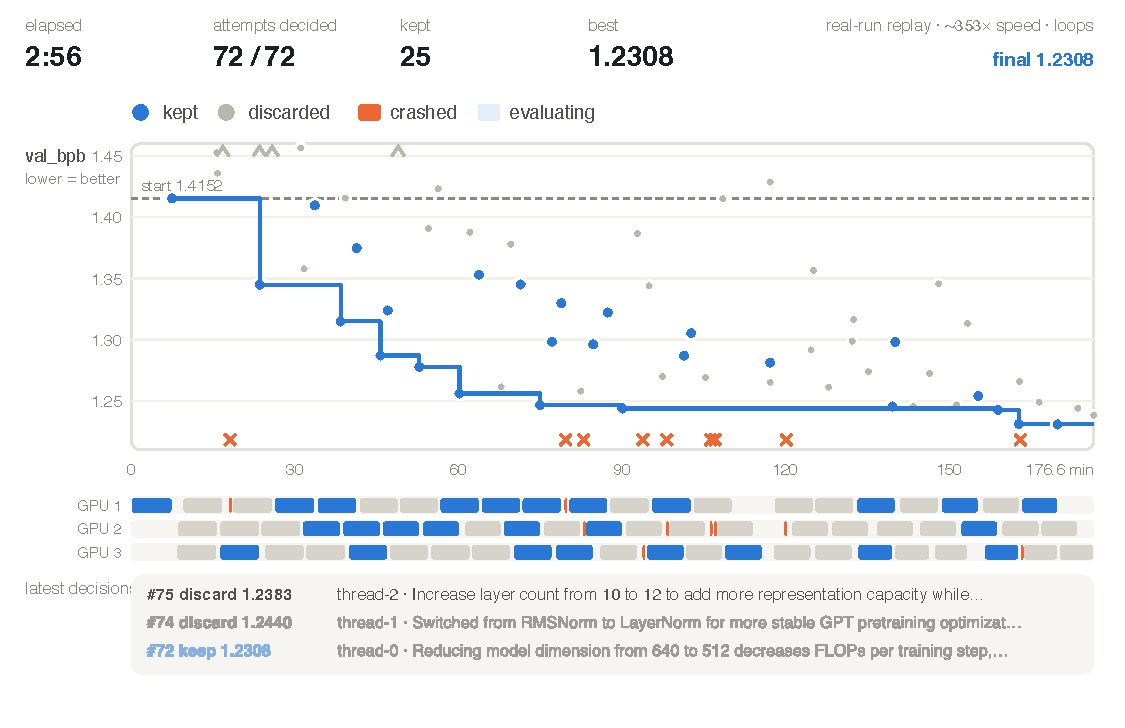
\includegraphics[width=0.6\linewidth]{figs/fig4-replay.pdf}
  \caption{Replay of the NanoChat research run, reconstructed from the event log. The top shows the best validation loss and individual evaluations, the middle shows parallel evaluations, and the bottom shows the model's decisions and proposals~\cite{replay-final-ovn1118b-nc-g0-events-jsonl,LOG-E}.}
  \label{fig:replay}
\end{figure}

\textbf{A fixed improver: clear first-order progress.} Qwen3.5-9B ran for 176.6 minutes and proposed and evaluated 72 attempts, lowering NanoChat validation loss by 0.1844, from 1.4152 to 1.2308 (Figure~\ref{fig:replay})~\cite{LOG-E}. Evaluation noise does not account for this change. The improver remained fixed, establishing first-order research progress; successor comparisons test whether research ability grows across generations.

\textbf{Lessons note: local experience became a general rule.} After reading records from eight training tasks, the model wrote a 252-word lessons note. It prescribed a fixed order for adjusting hyperparameters and advised: ``Ignore changes that increase loss even slightly.'' Adding the note to the prompt lowered improvement speed from 0.588 to 0.392, a difference of $-0.196$ (95\% CI $[-0.383, -0.033]$). Equal-length generic advice scored about 0.631; the lessons note trailed this control on all eight tasks, by a mean of $-0.239$ (95\% CI $[-0.420, -0.075]$, $p=0.008$)~\cite{decisions-decisions-1235-json}. This pattern is consistent with the note turning local successes on the training tasks into a fixed search order: the experience led the model to rule out potentially useful exploration earlier. Unverified experience did not transfer as a cross-task strategy in this experiment.

\textbf{Weight updates: accepted records did not beat rejected records.} Generation~1 was fine-tuned on research records accepted by the original model; its placebo was trained on an equal number of rejected records under the same settings. The two models were nearly identical on unseen tasks: Generation~1 was ahead by 0.004 (95\% CI $[-0.084, 0.080]$, $p=0.91$)~\cite{decisions-decisions-1235-json}. The comparison provides no evidence that accepted records taught the model to distinguish effective research hypotheses. Generations~2 and~3 tested whether an updated model could produce more useful records for the next successor; to control data volume, the successor and the original-model control received equal numbers of new records, generated by different models. The original model and the three successors scored 0.588, 0.537, 0.573, and 0.487. Generation~2 returned close to baseline, and Generation~3 scored 0.087 below Generation~2 (95\% CI $[-0.190, -0.005]$, sign-flip $p=0.0625$). No generation exceeded the original model~\cite{LOG-E,LOG-H,decisions-decisions-1235-json}.

\begin{figure}[t]
  \centering
  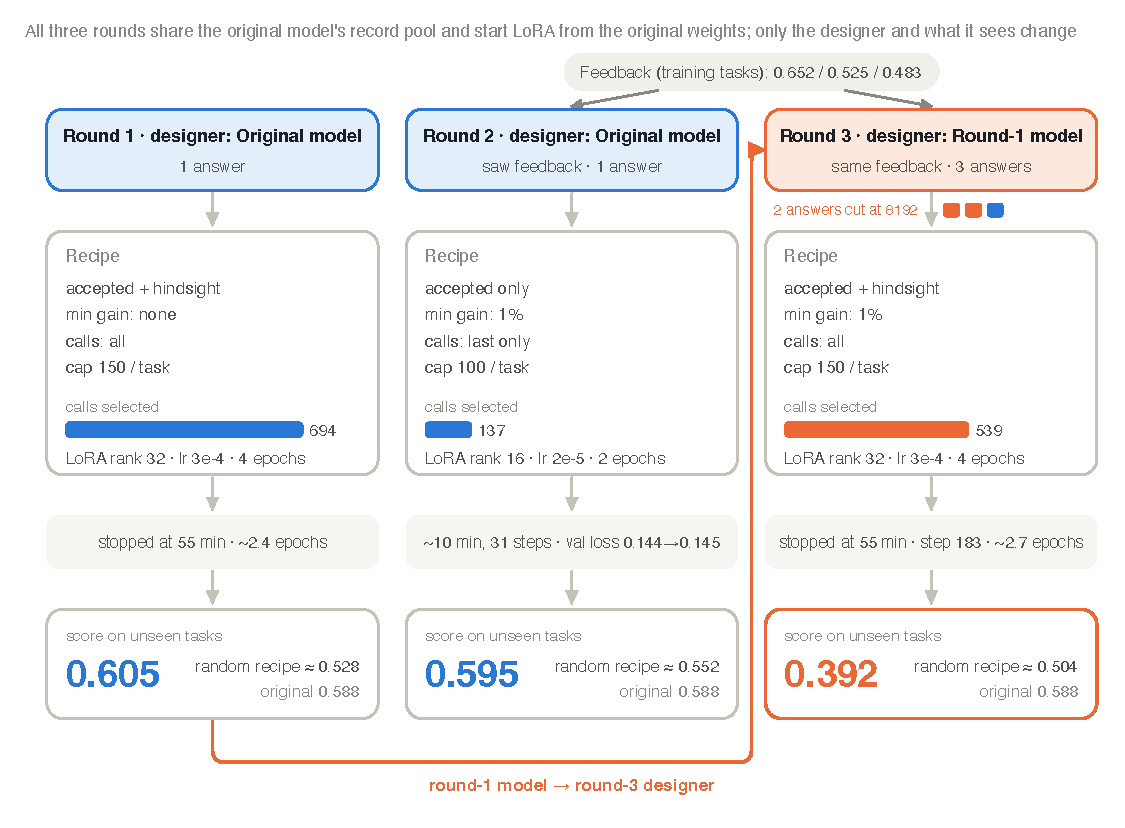
\includegraphics[width=0.72\linewidth]{figs/fig4-rounds.pdf}
  \caption{The designers, data filters, training settings, and unseen-task scores for the three self-designed recipes. Rounds 2 and 3 received the same feedback, but round 3's designer was the round-1 fine-tuned model~\cite{decisions-decisions-1235-json,decisions-decisions-1420-json}.}
  \label{fig:rounds}
\end{figure}

\textbf{Self-designed recipes: intuition did not identify a better update.} The model then chose data filters and LoRA settings from a predefined option space (Figure~\ref{fig:rounds}). The original model's first recipe scored 0.605, a second recipe designed after seeing one round of training-task feedback scored 0.595, and a third recipe designed by the first fine-tuned model scored 0.392. The third recipe scored 0.204 below the second (95\% CI $[-0.365, -0.065]$, $p=0.008$)~\cite{LOG-E,decisions-decisions-1235-json}. It resembled the first but added a filter that kept only records with at least 1\% relative gain. Retraining the first recipe with a new seed yielded 0.602, close to its original 0.605 (difference $-0.003$, $p=0.98$), so ordinary seed variation cannot explain the gap between rounds 1 and 3. Qwen3.8-27B used the same filter with lighter training and scored 0.513, above round 3 but below the original and round-2 models~\cite{LOG-E,decisions-decisions-1420-json}. Data selection and training intensity both shape successor performance. The successor’s improvement speed is the practical test of a proposed recipe.

\textbf{Continuing from the NanoChat frontier.} The original model, Generation~1, the rejected-record placebo, and the model with the lessons note each continued from the same best NanoChat checkpoint for 12 attempts, with three runs per group. Their mean loss reductions were 0.0124, 0.0203, 0.0178, and 0.0110; group differences were not statistically significant, and within-group variation across runs was substantial~\cite{decisions-cf-analysis-json}. In this setting too, successors showed no stable research-speed advantage.

\textbf{Interpretation.} Successful trajectories, free-text lessons, and self-designed recipes did not automatically produce stronger research ability. Data selection and training intensity change successor performance, so self-updates should be evaluated by putting the successor back into the improver role. Across this base model and task suite, no second-order acceleration was detected.

%=====================================================================
\section{Comparison with the literature}
\label{sec:lit}

Section~\ref{sec:exp} evaluates self-update signals by measuring successor research ability. Related studies examine task-score gains, agent-code modification, or faster improvement across generations; each measures a different outcome.

\textbf{Experience transfers only when it is validated.} The model-written lessons note lowered improvement speed, echoing negative results in studies of reflection and memory. ExpeL, Reflexion, and ACE report performance drops when reflections or context rewrites lack reliable external filtering~\cite{M-25,M-23,M-27}. Positive results tend to tie experience to verifiable artifacts: Sarukkai et al.\ retrieve successful trajectories, while Voyager stores executable skills that pass self-verification~\cite{M-28,M-24}. Transferable lessons need environmental validation and task-specific evidence.

\textbf{Accepted records did not teach research judgment.} The near-identity of Generation~1 and the rejected-record placebo resembles Spurious Rewards, where random rewards captured most of the gain of true rewards on MATH-500~\cite{M2-07}. Mind the Gap likewise found that some apparent first-round self-improvement came from better format following rather than task ability~\cite{M2-01}. The accepted-record model and rejected-record placebo performed almost identically. This control distinguishes generic effects of training from learning useful research signals, and the experiment found no faster research progress from accepted records.

\begin{figure}[t]
  \centering
  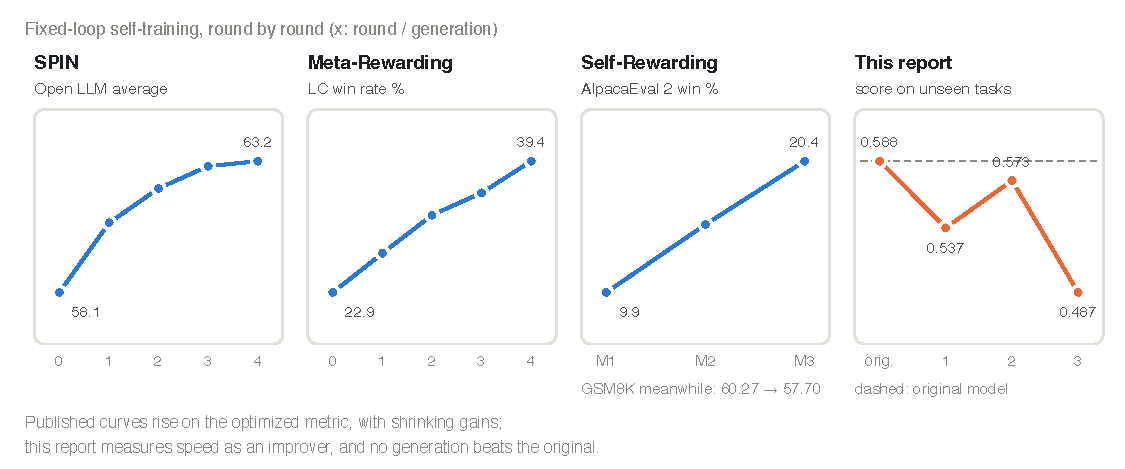
\includegraphics[width=0.66\linewidth]{figs/fig5-iter.pdf}
  \caption{Per-round task performance in self-training studies alongside the generational improvement-speed scores measured here. Each study retains its original metric; the panels show distinct measures and are not on a common scale~\cite{M-20,M-19,M-18,decisions-decisions-1235-json}.}
  \label{fig:iter}
\end{figure}

\textbf{Task scores and improvement ability measure different outcomes.} Many self-training studies report model performance on the target task. SPIN and Self-Rewarding show that some metrics continue to rise across iterations, while also reporting diminishing gains or regressions on other tasks (Figure~\ref{fig:iter})~\cite{M-20,M-18}. These findings describe changes in task performance; they do not directly test whether an updated model can improve the next task faster. Agent-level work offers adjacent but distinct evidence. DGM shows that letting an improved agent perform the next round of code edits can raise the final result~\cite{M-03}. AIDE$^2$'s ignition test directly compares an evolved coach with a hand-built coach, but does not distinguish them~\cite{E-28}. Their targets, update mechanisms, and budgets differ, so their scores cannot be compared numerically with weight-level improvement-speed scores. The fixed per-run budget also makes these scores distinct from the cumulative-input measure $r$~\cite{T-16,T-17}.

%=====================================================================
\section{A research direction for Ling}
\label{sec:ling}

Training Ling for recursive improvement requires feedback on whether each successor becomes a better improver. In this experiment, lessons notes and self-designed recipes did not increase successor improvement speed. Ling can propose updates and learn from independent evaluations of the resulting researcher. Ling-3.0-flash has a foundation for agent research: it is a MoE model with 124B total and 5.1B active parameters, trained with a large set of interactive environments~\cite{S-10}. Ant's Ring-1T reinforcement-learning system and AReaL asynchronous training framework offer infrastructure that could support the loop~\cite{S-12,S-13}.

\begin{figure}[t]
  \centering
  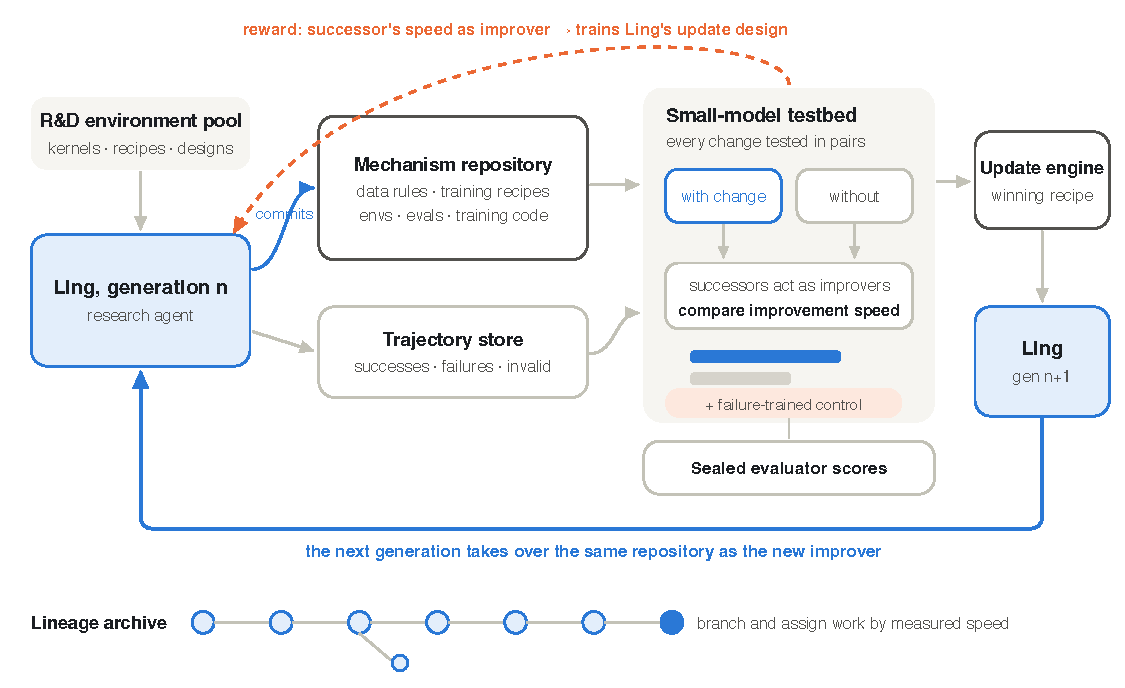
\includegraphics[width=0.72\linewidth]{figs/fig6-pipeline.pdf}
  \caption{Ling's research loop. Ling works on R\&D tasks and proposes changes to training data, update recipes, research environments, or evaluations. Candidate changes are tested independently; a change advances only when its successor improves faster on held-out tasks. Generational results also train Ling's ability to design updates. The lineage archive retains model weights, mechanism versions, and evaluation results.}
  \label{fig:pipeline}
\end{figure}

\textbf{Include improvement ability in the training objective.} The loop has four interdependent parts (Figure~\ref{fig:pipeline}): an \emph{R\&D task pool} covering training code, inference kernels, data processing, and recipe design, with held-out evaluations; a \emph{mechanism repository} that versions data rules, training recipes, environments, evaluators, and code, where Ling can propose changes and each change is traceable; \emph{independent evaluation} that measures whether a change produces a faster-improving successor, with fixed budgets, paired tasks, and sealed test data; and \emph{update and lineage}, which trains successors from evaluated changes and records weights, mechanism versions, data sources, and generational results. The key measurement follows Section~\ref{sec:exp}: train a candidate successor, put it back in the improver role, and compare it with a control on held-out R\&D tasks. The resulting feedback measures whether an update made the successor better at improving. DGM's self-modification framework, SEAL's outer-loop reinforcement learning, and AIDE$^2$'s ignition test offer components to build on~\cite{M-03,M-13,E-28}.

\textbf{Start with verifiable tasks.} Early tasks can prioritize clear evaluation signals, such as inference-kernel correctness and speed or training recipes under a fixed budget. Ling proposes a mechanism change, and the system constructs successors with and without that change under the same task and budget. Only reproducible positive results advance to training; failed and ineffective proposals remain available as controls. The objective should move from ``propose an update'' to ``propose an update that survives evaluation'': the reward should come from generational comparisons on independent tasks, so the model cannot simply optimize an evaluator that it wrote itself.

\textbf{What would count as progress.} Each Ling generation should be compared with its predecessor and a control on held-out R\&D tasks under a fixed budget, with task-paired improvement-speed scores, independent training runs, and uncertainty intervals. Repeated gains across tasks and random seeds would support the claim that Ling is getting better at improving. Task scores, the number of generated research records, and the model's own description of its progress cannot replace this measurement.

%=====================================================================
\begin{thebibliography}{99}
\small
\bibitem{E-28} Srikanth, Zhao, Xu, Wu, Jiang, Recursive self-improvement of AI research agents (AIDE², Weco AI, 2026-09). \url{https://arxiv.org/abs/2609.26457}
\bibitem{lit-rsi-academic-md} How academia treats RSI: summary of a review of about 96 sources. Project file \texttt{research/lit\_rsi\_academic.md}. \url{https://github.com/AlbertQiSun/rsi-report/blob/main/research/lit_rsi_academic.md}
\bibitem{LOG-E} RSI-mini experiment log, section E (results). Project file \texttt{research/REPORT\_LOG.md}. \url{https://github.com/AlbertQiSun/rsi-report/blob/main/research/REPORT_LOG.md#L37}
\bibitem{decisions-decisions-1420-json} Effects, 95\% CIs and permutation tests for every comparison (exported 11-18 14:20, incl. the two follow-up experiments). Project file \texttt{research/decisions/decisions\_1420.json}. \url{https://github.com/AlbertQiSun/rsi-report/blob/main/research/decisions/decisions_1420.json}
\bibitem{T-05} Schmidhuber (2003/2006), "Gödel Machines: Self-Referential Universal Problem Solvers Making Provably Optimal Self-Improvements", arXiv cs/0309048 v5. \url{https://arxiv.org/abs/cs/0309048}
\bibitem{T-12} Yampolskiy (2015), "From Seed AI to Technological Singularity via Recursively Self-Improving Software", arXiv 1502.06512. \url{https://arxiv.org/abs/1502.06512}
\bibitem{T-24} Tang, Ma, Li \& Yuan (2026), "Generalized Agent Iteration: One Formal Framework for Iterative Policy Improvement and Recursive Self-Improvement", arXiv 2609.13406 v2. \url{https://arxiv.org/abs/2609.13406}
\bibitem{T-01} I. J. Good (1965), "Speculations Concerning the First Ultraintelligent Machine", Advances in Computers 6. \url{https://www.stat.vt.edu/content/dam/stat_vt_edu/graphics-and-pdfs/research-papers/Technical_Reports/TechReport05-3.pdf}
\bibitem{T-23} ICLR 2026 Workshop on AI with Recursive Self-Improvement (Rio de Janeiro, 2026-04-26). \url{https://recursive-workshop.github.io/}
\bibitem{T-03} Yudkowsky (2008), "Recursive Self-Improvement", LessWrong. \url{https://www.lesswrong.com/posts/JBadX7rwdcRFzGuju/recursive-self-improvement}
\bibitem{T-09} Chalmers (2010), "The Singularity: A Philosophical Analysis", Journal of Consciousness Studies 17:7–65. \url{https://consc.net/papers/singularity.pdf}
\bibitem{T-08} Mahoney (2008, rev. 2010), "A Model for Recursively Self Improving Programs". \url{https://mattmahoney.net/rsi.pdf}
\bibitem{X-24} Weco AI. First evidence of recursive self-improvement. Company blog, 2026. \url{https://weco.ai/blog/first-evidence-of-recursive-self-improvement}
\bibitem{E-27} Wang et al. (incl. Schmidhuber), Huxley-Gödel Machine (2025-10). \url{https://arxiv.org/abs/2510.21614}
\bibitem{T-16} Besiroglu, Erdil \& Ho (2024), "Do the Returns to Software R\&D Point Towards a Singularity?", Epoch AI. \url{https://epoch.ai/blog/do-the-returns-to-software-rnd-point-towards-a-singularity}
\bibitem{T-17} Eth \& Davidson (2025), "Will AI R\&D Automation Cause a Software Intelligence Explosion?", Forethought. \url{https://www.forethought.org/research/will-ai-r-and-d-automation-cause-a-software-intelligence-explosion}
\bibitem{REL-RF} Recursive Superintelligence. First steps toward automated AI research. Company blog, 2026. \url{https://recursive.com/updates/first-steps-toward-automated-ai-research}
\bibitem{REL-NV} NaiveAI. Naive-N0.5-Flash: Building frontier AI with AI. Company research page, 2026. \url{https://naive.ai/en/research/}
\bibitem{REL-FL} Recursive Superintelligence. Introducing Flint. Company release, 2026. \url{https://recursive.com/updates/introducing-recursive-flint}
\bibitem{REL-AX} Apex Intelligence. Introducing Apex-35B-V1.0. Company release, 2026. \url{https://www.apexin.com/apex-35b/#ai}
\bibitem{E-01} Wijk et al., RE-Bench (METR, 2024-11; v2 2025-05). \url{https://arxiv.org/abs/2411.15114}
\bibitem{E-03} Chan et al., MLE-bench (OpenAI, 2024-10). \url{https://arxiv.org/abs/2410.07095}
\bibitem{E-04} Starace et al., PaperBench (OpenAI, 2025-04). \url{https://arxiv.org/abs/2504.01848}
\bibitem{E-23} Cunningham, Rush, Whitfill, Wijk, Independent Assessment of AI R\&D Acceleration at Anthropic in October 2026 (METR, 2026-11-05). \url{https://metr.org/blog/2026-11-05-anthropic-ai-rd-acceleration-assessment}
\bibitem{M-14} STaR: Zelikman, Wu, Mu, Goodman 2022. \url{https://arxiv.org/abs/2203.14465}
\bibitem{M-17} ReST-EM: Singh, Co-Reyes, Agarwal, et al. 2023. \url{https://arxiv.org/abs/2312.06585}
\bibitem{M-20} SPIN: Chen, Deng, Yuan, Ji, Gu 2024. \url{https://arxiv.org/abs/2401.01335}
\bibitem{M-01} STOP: Zelikman, Lorch, Mackey, Kalai 2023. \url{https://arxiv.org/abs/2310.02304}
\bibitem{M-03} Darwin Gödel Machine (DGM): Zhang, Hu, Lu, Lange, Clune 2025. \url{https://arxiv.org/abs/2505.22954}
\bibitem{M-04} Huxley-Gödel Machine (HGM): Wang, Piękos, Nanbo, …, Schmidhuber 2025. \url{https://arxiv.org/abs/2510.21614}
\bibitem{E-25} Zelikman et al., STOP: Self-Taught Optimizer (2023-10; v3 2024-08). \url{https://arxiv.org/abs/2310.02304}
\bibitem{E-33} Von Arx, Chan, Barnes, Recent Frontier Models Are Reward Hacking (METR, 2025-06). \url{https://metr.org/blog/2025-06-05-recent-reward-hacking/}
\bibitem{LOG-H} RSI-mini experiment log, section H (discussion and checks). Project file \texttt{research/REPORT\_LOG.md}. \url{https://github.com/AlbertQiSun/rsi-report/blob/main/research/REPORT_LOG.md#L204}
\bibitem{platform-design-md} RSI-mini platform design: definitions, decision rules and controls. Project file \texttt{research/platform\_design.md}. \url{https://github.com/AlbertQiSun/rsi-report/blob/main/research/platform_design.md}
\bibitem{decisions-decisions-1235-json} Effects, 95\% CIs and permutation tests for every comparison (exported 11-18 12:35, incl. round 3 of the self-designed recipe). Project file \texttt{research/decisions/decisions\_1235.json}. \url{https://github.com/AlbertQiSun/rsi-report/blob/main/research/decisions/decisions_1235.json}
\bibitem{replay-final-ovn1118b-nc-g0-events-jsonl} Event log of the Qwen3.5-9B research run on NanoChat (proposals, evaluations, decisions). Project file \texttt{research/replay/final/ovn1118b-nc-g0/events.jsonl}. \url{https://github.com/AlbertQiSun/rsi-report/blob/main/research/replay/final/ovn1118b-nc-g0/events.jsonl}
\bibitem{decisions-cf-analysis-json} Continue-from-best: drops and comparisons for four improvers, 3 runs each. Project file \texttt{research/decisions/cf\_analysis.json}. \url{https://github.com/AlbertQiSun/rsi-report/blob/main/research/decisions/cf_analysis.json}
\bibitem{M-25} ExpeL: Zhao, Huang, Xu, Lin, Liu, Huang 2023. \url{https://arxiv.org/abs/2308.10144}
\bibitem{M-23} Reflexion: Shinn, Cassano, Berman, Gopinath, Narasimhan, Yao 2023. \url{https://arxiv.org/abs/2303.11366}
\bibitem{M-27} ACE: Zhang, Hu, Upasani, et al. 2025. \url{https://arxiv.org/abs/2510.04618}
\bibitem{M-28} Self-generated in-context examples: Sarukkai, Xie, Fatahalian 2025. \url{https://arxiv.org/abs/2505.00234}
\bibitem{M-24} Voyager: Wang, Xie, Jiang, et al. 2023. \url{https://arxiv.org/abs/2305.16291}
\bibitem{M2-07} Spurious Rewards (Shao et al. 2025, arXiv 2506.10947). \url{https://arxiv.org/abs/2506.10947}
\bibitem{M2-01} Mind the Gap (Song, Zhang, Eisenach, Kakade, Foster, Ghai 2024, arXiv 2412.02674). \url{https://arxiv.org/abs/2412.02674}
\bibitem{M-19} Meta-Rewarding: Wu, Yuan, Golovneva, Xu, Tian, Jiao, Weston, Sukhbaatar 2024. \url{https://arxiv.org/abs/2407.19594}
\bibitem{M-18} Self-Rewarding LMs: Yuan, Pang, Cho, Li, Sukhbaatar, Xu, Weston 2024. \url{https://arxiv.org/abs/2401.10020}
\bibitem{S-10} inclusionAI. Ling-3.0-flash model card and config. Hugging Face, 2026 (self-reported). \url{https://huggingface.co/inclusionAI/Ling-3.0-flash}
\bibitem{S-12} Ling Team, "Every Step Evolves: Scaling Reinforcement Learning for Trillion-Scale Thinking Model" (Ring-1T), arXiv:2510.18855. \url{https://arxiv.org/abs/2510.18855}
\bibitem{S-13} Fu et al., "AReaL: A Large-Scale Asynchronous Reinforcement Learning System for Language Reasoning", arXiv:2505.24298. \url{https://github.com/inclusionAI/AReaL}
\bibitem{M-13} SEAL: Zweiger, Pari, Guo, Akyürek, Kim, Agrawal 2025. \url{https://arxiv.org/abs/2506.10943}
\end{thebibliography}


\end{document}
